\documentclass[conference]{IEEEtran}
%\IEEEoverridecommandlockouts
% The preceding line is only needed to identify funding in the first footnote. If that is unneeded, please comment it out.
\usepackage{todonotes}
\usepackage{cite}
\usepackage{array, booktabs, makecell} % For formal tables
\usepackage{algorithm,algpseudocode}
\usepackage{adjustbox}
\usepackage{graphicx}
\usepackage{textcomp}
\usepackage{xcolor}
\usepackage{listings}
\usepackage{hyperref}
\newcommand{\RomanNumeralCaps}[1]{\MakeUppercase{\romannumeral #1}}
\usepackage{url}
\usepackage{enumitem}
\usepackage{amsmath, amsthm, amssymb, amsfonts}
\usepackage{tikz}
\usepackage{stfloats}
\usepackage{pifont}
\newcommand{\cmark}{\ding{51}}%
\newcommand{\xmark}{\ding{55}}

\newtheorem{property}{Property}

\usetikzlibrary{arrows,automata,shapes,positioning}
\tikzset{
	normal/.style = {
		rectangle split, 
		rectangle split parts=2, 
		very thick, draw=black, 
	}
}

\definecolor{vdarkgreen}{rgb}{0,0.3,0}
\lstset{
	language=Java,
	columns=flexible,
	numbers=left,
        numbersep=2pt,
	stepnumber=1,
	keywordstyle=\color{blue},
	tabsize=1,
    keywordstyle=\color{blue}\bfseries,
    commentstyle=\color{vdarkgreen},
    stringstyle=\ttfamily\color{red!50!brown},
        showstringspaces=false}
\lstset{literate=%
    *{0}{{{\color{red!20!violet}0}}}1
    {1}{{{\color{red!20!violet}1}}}1
    {2}{{{\color{red!20!violet}2}}}1
    {3}{{{\color{red!20!violet}3}}}1
    {4}{{{\color{red!20!violet}4}}}1
    {5}{{{\color{red!20!violet}5}}}1
    {6}{{{\color{red!20!violet}6}}}1
    {7}{{{\color{red!20!violet}7}}}1
    {8}{{{\color{red!20!violet}8}}}1
    {9}{{{\color{red!20!violet}9}}}1
}

\def\BibTeX{{\rm B\kern-.05em{\sc i\kern-.025em b}\kern-.08em
    T\kern-.1667em\lower.7ex\hbox{E}\kern-.125emX}}
\begin{document}
\bstctlcite{IEEEexample:BSTcontrol}

\title{MockDetector: Detecting and tracing mock objects in unit tests}

% \author{\IEEEauthorblockN{Qian Liang, Patrick Lam}
% \IEEEauthorblockA{\textit{Department of Electrical and Computer Engineering} \\
% \textit{University of Waterloo}\\
% Waterloo, Canada \\
% \{q8liang, patrick.lam\}@uwaterloo.ca}
% }
%% \and
%% \IEEEauthorblockN{3\textsuperscript{rd} Given Name Surname}
%% \IEEEauthorblockA{\textit{dept. name of organization (of Aff.)} \\
%% \textit{name of organization (of Aff.)}\\
%% City, Country \\
%% email address or ORCID}
%% \and
%% \IEEEauthorblockN{4\textsuperscript{th} Given Name Surname}
%% \IEEEauthorblockA{\textit{dept. name of organization (of Aff.)} \\
%% \textit{name of organization (of Aff.)}\\
%% City, Country \\
%% email address or ORCID}
%% \and
%% \IEEEauthorblockN{5\textsuperscript{th} Given Name Surname}
%% \IEEEauthorblockA{\textit{dept. name of organization (of Aff.)} \\
%% \textit{name of organization (of Aff.)}\\
%% City, Country \\
%% email address or ORCID}
%% \and
%% \IEEEauthorblockN{6\textsuperscript{th} Given Name Surname}
%% \IEEEauthorblockA{\textit{dept. name of organization (of Aff.)} \\
%% \textit{name of organization (of Aff.)}\\
%% City, Country \\
%% email address or ORCID}
%% }

\maketitle

\begin{abstract}
	Software dependencies are ubiquitous and may pose problems during testing, because creating usable objects from dependencies is often complicated.
	Developers, therefore, often introduce mock objects to stand in for dependencies during testing. However, to our knowledge, no static analysis framework provides a tool to automatically identify mock objects created in the unit test cases. The lack of mock object detection can decrease the precision of static analyses, as they are unable to separate methods invoked on mock objects from methods invoked on actual objects. 
	
	In this paper, we introduce MockDetector, a technique to identify mock objects. It is able to detect common Java mock libraries' APIs that create mock objects, checking whether there is a call to a mock creation site, followed by a forward flow must analysis, which aims to include all locals that are indeed mock objects on all possible paths, as well as the containers such as array or collection that have must mock objects stored. Implications of understanding which objects are mock objects include helping static analysis tools identify which dependencies' methods are actually tested, versus mock methods being called.

\end{abstract}


\begin{IEEEkeywords}
Static Analysis, Dataflow Analysis, Declarative Program Analysis, Mock Objects, Unit Tests
\end{IEEEkeywords}

\section{Introduction}
\label{sec:introduction}

Mock objects ~\cite{beck02:_test_driven_devel} are a common idiom in
unit tests for object-oriented systems.  They allow developers to test objects that 
rely on other objects, likely from different components, or are simply complicated 
to build for testing purposes (e.g. a database).

While mock objects are an invaluable tool for developers, their use
complicates the static analysis of test cases. 
By design, a call to a mock object resembles a call to the real object. 
A naive static analysis attempting to be sound will have to include all of 
the possible behaviours of the actual object when analysing such code. 
As a result, such analysis would be useless in capturing the true behaviour 
of the test case.

Others have defined the notion of a focal method for a test case---the method
whose behaviour is being tested. ~\cite{7335402}
The test case would set up mock objects to provide parameters to this focal method.
When analyzing the test case, it would be useful to know which variables in the
method contain mock objects, in order to build a more precise call graph and get 
better insight of the overall project.

We have designed a helper static analysis, \textsc{MockDetector}, which identifies
mock objects in test cases. It starts from a list of mock object creation sites; we
have provided APIs for the common mocking libraries. It then propagates the mockiness
intraprocedurally through a forward flow must analysis and to containers, so that an analysis
can ask whether a given variable in a test case contains a mock or not. Currently, we have
evaluated \textsc{MockDetector} on a suite of 3 benchmarks. Manual inspection have shown 
correct intraprocedural mock detection over the benchmarks. 

Taking a broader view, we believe that helper static analyses can aid
in the development of more useful static analyses. These analyses can
encode useful domain properties; for instance, in our case, properties
of test cases. By taking a domain-specific approach, analyses can extract
useful facts about programs that would otherwise be difficult to establish.

We make the following contributions in this paper:
\begin{itemize}
\item We designed and implemented two variants of a static mock detection algorithm, one as a dataflow analysis implemented imperatively (using Soot) and the other declaratively (using Doop).
\item We evaluate both the relative ease-of-implementation and precision of the imperative and declarative approaches, both intraprocedurally and interprocedurally. % potentially intraprocedural as well
\item Using our tool, we characterize the prevalence of mock objects in the test suites for a total of 8 open-source benchmarks along with out microbenchmark consisting of 184K lines of code, finding that 981 out of 6282 unit tests use (intra) mock objects, and that there are a total of 1811 method invocations on mock objects.
\end{itemize}
At a higher level, we see this paper as making both a contribution and a meta-contribution to
problems in source code analysis. The contribution, mock detection, enables more accurate analyses
of test cases, which account for a signficant fraction of modern codebases. The meta-contribution,
comparing analysis approaches, will help future researchers decide how to best solve their
source code analysis problems.

\section{Motivating Example}
\label{sec:motivating-example}

In this section, we illustrate how \textsc{MockDetector} finds a mock object created within a unit test case. Our tool identifies variables which have been assigned an object flowing from a mock creation site either using a forward dataflow may-analysis (Soot-based analysis) or by solving specified declarative constraints (Doop-based analysis).

% explain focal methods first.

To motivate our work, consider Listing~\ref{lis:mockCall}, which presents a unit test case from the Maven project. Line 8 calls \textit{getRequest()}, invoking it on the mock object \texttt{session}. Line 12 then calls \textit{getToolchainsForType()}---this is the actual focal method whose behaviour is being tested. At the bytecode level, the two method invocations are indistinguishable with respect to mockness; to our knowledge, current static analysis tools cannot easily tell the difference between the method invocation on a mock object on line~\ref{line:mock} and the method invocation on a real object on line~\ref{line:real}. An IDE with information about mock invocations could provide better suggestions around it. And the uncertainty would confound a naive static analysis that attempts to identify focal methods. For instance, Ghafari et al~\cite{ghafari15:_autom}'s heuristic would fail on this test, as it returns the last mutator method in the object under test, and the focal method here is an accessor. 

Figure~\ref{fig:focalMethodIllustration} shows how our analysis tool marks mock calls as not being potential focal method calls.

[NEED BETTER EXPLANATION OF WHAT IS HAPPENING IN FIGURE 1 INCLUDING DISCUSSION OF THE ABSTRACTION]

While we were designing \textsc{MockDetector}, we observed several cases where developers store mock objects in arrays and collections. Listing~\ref{lis:container} presents method \textit{setUp()} in class \texttt{NodeListIteratorTest.java} from commons-collections-4.4, where line \ref{line:storeMocksInArray} puts the mock \texttt{Node} objects in the array-typed field \texttt{nodes}, which is later used in test cases. To find arrays containing mock objects, our analysis would first locate assignment statements containing array references, and would gather all the local variables or field references which appear as sources in these statements. It then checks whether any of these local variables or field reference sources have been marked as mock objects in the analysis. If so, then the tool would mark the local variable or field reference representing the array as an array mock---it propagates the mockness to this array container. Figure~\ref{fig:arrayMockIllustration} illustrates the process of identifying mock-containing containers.

[SAME FOR FIGURE 2]

\lstset{language=java,
    keywordstyle=\color{blue}\bfseries,
    commentstyle=\color{green},
    stringstyle=\ttfamily\color{red!50!brown},
        showstringspaces=false}
\lstset{literate=%
    *{0}{{{\color{red!20!violet}0}}}1
    {1}{{{\color{red!20!violet}1}}}1
    {2}{{{\color{red!20!violet}2}}}1
    {3}{{{\color{red!20!violet}3}}}1
    {4}{{{\color{red!20!violet}4}}}1
    {5}{{{\color{red!20!violet}5}}}1
    {6}{{{\color{red!20!violet}6}}}1
    {7}{{{\color{red!20!violet}7}}}1
    {8}{{{\color{red!20!violet}8}}}1
    {9}{{{\color{red!20!violet}9}}}1
}

\begin{lstlisting}[basicstyle=\ttfamily, caption={This code snippet illustrates an example from maven-core, where both the focal method \texttt{getToolchainsForType} and a method invocation \texttt{getRequest} on a mock object occur in test \textit{testMisconfiguredToolchain()}},
basicstyle=\scriptsize\ttfamily,language = Java, framesep=4.5mm, escapechar=|,
framexleftmargin=1.0mm, captionpos=b, xleftmargin=3.5ex, label=lis:mockCall]
@Test
public void testMisconfiguredToolchain()
                 throws Exception {
    MavenSession session = mock( MavenSession.class );
    MavenExecutionRequest req = 
        new DefaultMavenExecutionRequest();
    when( session.getRequest() ).thenReturn( req ); |\label{line:mock}|
    
    ToolchainPrivate[] basics =
         toolchainManager.getToolchainsForType("basic", session); |\label{line:real}|
    
    assertEquals( 0, basics.length );
}
\end{lstlisting}

\begin{lstlisting}[basicstyle=\ttfamily, caption={This example illustrates a field array container holding mock objects from \textit{setup()} in \texttt{NodeListIteratorTest.java}.},
basicstyle=\scriptsize\ttfamily,language = Java, framesep=4.5mm, framexleftmargin=1.0mm, captionpos=b, xleftmargin=3.5ex, label=lis:container, escapechar=|]
// Node array to be filled with mock Node instances
private Node[] nodes;

@Test
protected void setUp() throws Exception {
    // ...

    // create mock Node Instances and 
    // fill Node[] to be used by test cases
    final Node node1 = createMock(Element.class);
    final Node node2 = createMock(Element.class);
    final Node node3 = createMock(Text.class);
    final Node node4 = createMock(Element.class);
    nodes = new Node[] {node1, node2, node3, node4}; |\label{line:storeMocksInArray}|
    // ...
}
\end{lstlisting}


\begin{figure}
    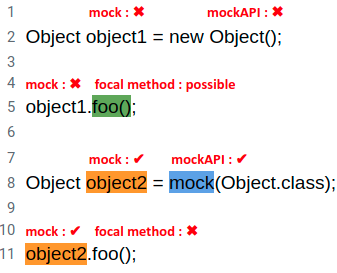
\includegraphics[width=.25\textwidth]{Images/mockFocalMethodIllustration.png}
    
    \caption{Illustration of the process locating mock object and determining non focal method.}
    \label{fig:focalMethodIllustration}
    
\end{figure}

\begin{figure}
    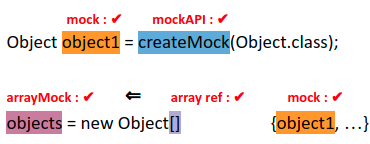
\includegraphics[width=.25\textwidth]{Images/arrayMockIllustration.png}
    
    \caption{Illustration of the process determining array that is an arrayMock.}
    \label{fig:arrayMockIllustration}
    
\end{figure}

\section{Technique}
\label{sec:technique}

We present two complementary ways of statically computing mock information: an imperative implementation of a dataflow analysis (using the Soot~\cite{Vallee-Rai:1999:SJB:781995.782008} program analysis framework), along with a declarative implementation (using the Doop~\cite{bravenboer09:_stric_declar_specif_sophis_point_analy} framework). We started this project with the usual imperative approach to implementing a static analysis---in our context, that meant using Soot. Then, when we wanted to experiment with adding more features to the analysis, we decided that this was a good opportunity to learn about Doop's declarative approach as well. We added new features to the Doop implementation and backported them to the Soot implementation. While the core analysis is similar, the different implementation technologies have different affordances. For instance, it is easier for the Doop version to mark a field as mock-containing than for the Soot version to do so. In Section~\ref{sec:evaluation}, we compare the results obtained using each technology.

\subsection{Common Infrastructure}
We have parameterized our technique with respect to mocking libraries and have instantiated it with respect to the popular Java libraries Mockito\footnote{\url{https://site.mockito.org/}}, EasyMock\footnote{\url{https://easymock.org/}}, and PowerMock\footnote{\url{https://github.com/powermock/powermock}}. We also support different versions of JUnit\footnote{\url{https://junit.org}}: 3, and 4+. We discuss the parameterization in this subsection.

Both JUnit and mocking libraries are highly-reflective and would normally pose problems for static analyses. Fortunately, they use reflection in limited, stylized ways, and we have designed our analyses to soundly handle these libraries.

\paragraph{JUnit and Driver Generation}
JUnit tests are simply methods that developers write in test classes, appropriately annotated (in JUnit 3 by method name starting with ``test'', in 4+ by a \texttt{@Test} annotation). A JUnit test runner uses reflection to find tests. Out of the box, static analysis engines do not see tests as reachable code.

% what about hierarchical drivers?

Thus, to enable static analysis over a benchmark's test suite, our tool uses Soot to generate a driver class for each Java sub-package of the suite (e.g. \texttt{org.apache.ibatis.executor.statement}). In each of these sub-package driver classes, our tool creates a \textit{runall()} method, which invokes all methods within the sub-package that JUnit (either 3 or 4) considers to be public, as well as non-constructor test cases, all surrounded by calls to class-level init/setup and teardown methods. Concrete test methods are particularly easy to call from a driver, as they are specified to have no parameters and are not supposed to rely on any particular ordering. 
Our tool then creates a RootDriver class at the root package level, which invokes the \textit{runall()} method in each sub-package driver class, along with the Test/Before/After methods created for the classes located at the root level. The drivers that we generate also contain code to catch all checked exceptions declared to be thrown by the unit tests. Both our Soot and Doop implementations use the generated driver classes.

All static frameworks must somehow approximate the set of entry points as appropriate for their targets. For instance, the Wala framework~\cite{wala19:_t} also creates synthetic entry points, but it does this to perform pointer analysis on a program's main code rather than to enumerate the program's test cases.

\paragraph{Intraprocedural Analysis} The Soot analysis is intraprocedural and the Doop analysis has an intraprocedural version. In both of these cases, we make the unsound (but reasonable for our anticipated use case) assumption that mockness can be dropped between callers and callees: at method entry points, no parameters are assumed to be mocks, and at method returns, the returned object is never a test. Doop's interprocedural version drops this assumption and instead context-insensitively propagates information from callers to callees and back; we discuss the results of doing so in Section~\ref{sec:evaluation}.

Call graphs are useful to our analysis in two ways: first, because they come with entry points (which we approximate directly in our context, as explained above); and second, because they help identify calls to mock source methods. We assume that developers do not call inherited versions of mock creation sites (though again, if a call graph is available in Doop, we use it).

\paragraph{Mock Libraries}
Our supported mock libraries take different approaches to declaring mocks. All of the libraries have methods that generate mock objects; for instance, EasyMock contains the \texttt{createMock()} method. We consider return values from these methods to be mock objects. Additionally, Mockito contains a fluent \texttt{verify()} method which returns a mock object. Finally, Mockito also allows developers to mark fields as \texttt{@Mock}; we treat reads from such fields as mock objects. Both implementations start the analysis by using these hard coded these facts on mock source methods, as described in the mock libraries' documentation.

\subsection{Imperative Soot Implementation}
We continue with describing each implementation in turn. In this subsection, we describe the Soot-based imperative dataflow analysis to find mock invocation sites. Our tool tracks information from the creation sites through the control-flow graph using a forward dataflow may-analysis---an object is declared a mock if there exists some execution path where it may receive a mock value. Our implementation also understands containers like arrays and collections, and tracks whether containers holds any mock objects. The abstraction marks all the contents of an array or container as potential mocks if it observes any mock object being put into the array or container.

% Mock Libraries discussed in Common Infrastructure section
%\paragraph{Define Common Mocking Library APIs}
%\label{subsubsec:collection}

%Our tool stores a pool of common APIs, provided by the analysis designer, which are used to create mock objects when using popular Java mocking libraries, including Mockito, EasyMock, and PowerMock. These APIs are the possible mock creation sites, where the locals/variables holding mock objects are first created.

%Given a pool of possible APIs to search for, our tool may analyze tests for their usage of these APIs.% Facts for mock source methods is discussed in doop, maybe this part could be discussed once to avoid repetition?


\paragraph{Forward Dataflow May Analysis}
\label{subsubsec:forward}

%To solve the problem, our tool uses forward may analysis, where it analyzes statements from top to bottom, and to keep variables that are verified to be mocks on any possible path at merged points. \textsc{MockDetector} uses the abstraction 
Our forward dataflow analysis maps values (locals and field references) in the Jimple intermediate representation to our abstraction:
\[ \mathtt{Value} \mapsto \mathtt{MockStatus}. \]
\texttt{MockStatus} records three bits: one for the value being a mock, one for it being an array containing a mock, and one for it being a collection containing a mock. At most one of the three bits may be true for any given value. Not having a mapping in the abstraction is equivalent to mapping to a MockStatus having all three bits false. Our tool would store a value with MockStatus holding three false bits into the abstraction if and only if the value was once a mock or mock-containing container, but later redefined to a non-mock object or container without mock objects.

We chose to implement a may-analysis rather than a must-analysis for two reasons: 1) we did not observe any cases where a value was assigned a mock on one branch and a real object on the other branch; 2) implementing a must-analysis would not help heuristics to find focal methods, as a must-analysis would rule out fewer mock invocations. Our merge operation is therefore a fairly standard pointwise disjunction of the two incoming values in terms of values and in terms of the 3 bits of \texttt{MockStatus}.

%% \textsc{MockDetector} implements the "may" logic in the following manner: it checks the two in-flows 
%% of \begin{lstlisting}[basicstyle=\ttfamily\small,numbers=none]
%% Map<Value, MockStatus>
%% \end{lstlisting}
%% from two paths. For any variable that is only stored in one map, the key-value pair is directly passed to the out-flow map. For a variable that is a shared key of the two maps, the analysis would update the out-flow's MockStatus by applying the "OR" operation on the "May Mock", "Array Mock", and "Collection Mock" bits from the MockStatus value retrieved from both in-flow maps. 

%% For each statement in a forward flow analysis, we consider two sets: generated set and killed set. In this study, the first set contains the locals that are judged to become mocks, whereas the killed set containing locals that are determined to no longer to be mocks. Equations (1) and (2) illustrates how the inflow and outflow are defined and calculated for each unit: $In(u)$, representing a program point before executing $u$, is the intersection of all outflows after executing each element in immediate predecessor statements of $u$; $Out(u)$, on the other hand, is determined by first removing the killed set from $In(u)$, and union the result with generated set. 

%% \begin{equation}
%% \mathrm{In}(u) = \bigcap_{u' \in preds(u)} \mathrm{Out}(u') 
%% \end{equation}

%% \begin{equation}
%% \mathrm{Out}(u) = (\mathrm{In}(u) - \mathrm{Kill}(u)) \bigcup \mathrm{Gen}(u) 
%% \end{equation}

Our dataflow analysis uses fairly standard gen and kill sets in the flow function. We set bits in \texttt{MockStatus} in the following cases:
%For the gen set, we consider for the Values in the following scenarios to be included in the abstraction, with mock bit set to 1:

First, the gen set includes pre-analyzed fields containing mock objects defined via annotation (e.g. \texttt{@Mock}), inside a constructor \texttt{<init>}, or in JUnit's \texttt{@Before}/\texttt{setUp()} methods. We discuss the pre-analysis below in Section~\ref{subsubsec:pre-analysis}. 

Second, it includes local variables assigned from mock-creation source methods:
\begin{lstlisting}[basicstyle=\ttfamily\small,numbers=none]
    X x = mock(X);
\end{lstlisting}
Third, it includes values assigned from return values of read methods from mock-containing collections or their array counterparts:
\begin{lstlisting}[basicstyle=\ttfamily\small,numbers=none]
    // array read;
    // r1 is in the in set as an array mock
    X x = r1[0];
    // collection read;
    // r2 is in the in set as a collection mock
    X x = r2.get(0);
\end{lstlisting}
Fourth, if \texttt{x} is a mock and casted and assigned to \texttt{x\_cast}, then the gen set includes \texttt{x\_cast} (e.g. \texttt{r1} in Listing~\ref{lis:arrayIllustrationIR}):
\begin{lstlisting}[basicstyle=\ttfamily\small,numbers=none]
    // x is in the in set as a mock
    X x_cast = (X) x;
\end{lstlisting}
Finally, the gen set includes copies of already-flagged mocks:
\begin{lstlisting}[basicstyle=\ttfamily\small,numbers=none]
    // x is in the in set with mock bit on
    X y = x;
\end{lstlisting}
The copy-related rules also apply to mock-containing arrays and collections, but we add some additional rules for generating mocks that the program reads from collections and arrays, as well as rules for marking arrays and collections as mock-containing.

For instance, in the below example, \texttt{r1} will be included in the gen set as an array mock, since it invokes an array write method, and \texttt{r2} (to be stored in the array) is a mock object as indicated in the in set. Similarly, \texttt{\$r4} will be added to the gen set as a collection mock, as it invokes an \texttt{ArrayList}'s write method, and \texttt{r3}, the object added to the ArrayList, is a known mock object.
\begin{lstlisting}[basicstyle=\ttfamily\small,numbers=none]
    // r2 is in the in set as a mock
    r1[0] = r2;
    // r3 is in the in set as a mock
    $r4.<java.util.ArrayList: boolean
             add(java.lang.Object)>(r3);
\end{lstlisting}

% nah, we say that above now.
%% In a similar fashion, the gen set will include values that traverse the program's control-flow graph via assignments, from a value that already has mock-containing array or mock-containing collection bit set to true.

%% \begin{lstlisting}[basicstyle=\ttfamily\small,numbers=none]
%% // arr2 is already in the gen set 
%% // with mock-containing array bit on.
%% arr1 = arr2
%% // arr2 is already in the gen set 
%% // with collection containing mock bit on.
%% collection1 = collection2
%% \end{lstlisting}

%% ---------

%% In our analysis, the generated set consists of two steps. Consider the statement: 
%% \begin{lstlisting}[basicstyle=\ttfamily\small,numbers=none]
%% Employee employee = mock(Employee.class);
%% \end{lstlisting}
%% The intermediate representation generated in Jimple format would be:
%% \begin{lstlisting}[basicstyle=\ttfamily\small,numbers=none]
%% $r1 = staticinvoke <org.mockito.Mockito: 
%% java.lang.Object mock(java.lang.Class)>
%% (class "Lca/liang/Employee;")

%% r2 = (ca.liang.Employee) $r1
%% \end{lstlisting}W

%% In this example, $\$r1$ is the immediate receiver from Mockito's mock creation site, whereas $r2$ is the casted expression that gets carried along in the subsequent program. Thus, our tool would include the immediate receivers, and the casted expressions of mock objects into the generation set, in two steps. 

\paragraph{Interprocedural support} The Heros framework\cite{bodden12:_inter_proced_data_flow_analy} implements IFDS/IDE for program analysis frameworks including Soot. With some effort, it would be possible to rewrite our mock analysis with Heros; however, this would be a more involved process than simply adding a line to the declarative analysis, as described below. In particular, Heros uses a different API in its implementation than does Soot. However, conceptually, it should be no harder to implement an interprocedural Heros analysis than a intraprocedural Soot dataflow analysis.

\paragraph{Containers} Several test suites use arrays or collection objects to hold mock objects. In this scenario, our tool would consider that mockness propagates out to the container. For instance, say the flow function encounters an array write \begin{lstlisting}[basicstyle=\ttfamily\small,numbers=none]
    r1[0] = r2
\end{lstlisting} 
Then, the tool will look for \texttt{r2} in the abstraction. Once the abstraction pinpoints \texttt{r2} (with mock bit on), it will include \texttt{r1} with mock-containing array bit set to true. (THIS PART STILL FEELS REPETITIVE.)


Taking an array as an example, our tool would first look for an array reference in the executing statement, meaning there is a read or a write from an array. If the effect is a STORE to the array, \textsc{MockDetector} would look for variables stored into the array, and check whether any of the variables have been found to be mocks. If so, it would label the array as an array mock, and set the relevant bit in the abstraction to true. Reversely, if is a LOAD effect from the array, \textsc{MockDetector} would check if the array itself has mock-containing array bit on in the abstraction. If so, it will mark the value assigned from the array LOAD with mock bit on, and store it in the abstraction.

*** we say more about collections in the related work, we should probably move that to here.

We treat collections analogously. The main difference is Java's \texttt{Collection} interface has multiple implementations, which expose different APIs for objects. \textsc{MockDetector} resolves this problem with a manually-constructed pool of read and write method APIs associated with each sub-type of the interface \texttt{java.util.Collection}. It subsequently checks (using the hierarchy) whether collection classes appear in statements containing invoke expression. This is achieved by first determining the declaring class of the invoked method. If the declaring class is of an interface, \textsc{MockDetector} would check whether \texttt{java.util.Collection} is a super-interface for the declaring class. Otherwise, if the declaring class is of a class type, \textsc{MockDetector} would check whether \texttt{java.util.Collection} is a super-interface for any of declaring class's implemented interfaces. If a collection sub-type container is presented, \textsc{MockDetector} would then check if a STORE effect is applied to the container, indicating some object is to be stored in the container. Once the object is determined to be a mock, the collection container variable would immediately be labelled as a collection mock, setting the relevant bit in the abstraction to true. Reversely, if a LOAD effect is applied to the container labelled as a collection mock, the object retrieved from the container will be labelled a mock, and setting the mock bit in the abstraction to true.

\subsubsection{Pre-Analysis for Field Mocks Defined in Constructors and Before Methods}
\label{subsubsec:pre-analysis} A number of our benchmarks define fields as mock objects via EasyMock or Mockito \texttt{@Mock} annotations, or initialize these fields in the \texttt{<init>} constructor or \texttt{@Before} methods (\textit{setUp()} in JUnit 3), which run before any test methods from those classes. These mock field or mock-containing container fields are then used in tests. In the Soot implementation, we use two pre-analyses before running the main analysis, under the assumption that fields are rarely, and not correctly, mutated in the test cases. (We have validated our assumption on benchmarks. Table~\ref{tab:mutations} shows a preliminary analysis of field mutation frequency inside test cases---fewer than 0.3\% of fields are mutated in test cases.)  

The first transformer handles annotated field mocks and field mocks defined in the constructors (\texttt{<init>} methods), while the second transformer handles \texttt{@Before} and \texttt{setUp()} methods. These transformers are implemented similarly.

\textsc{MockDetector} retrieves all fields in all test classes, and marks fields annotated {\tt Lorg/mockito/Mock;} or {\tt Lorg/easymock/Mock;} to its set of annotated mocks. \textsc{MockDetector} will store the three fields with \texttt{@Mock} into a HashSet, which later to be used in the main analysis.
% obvious enough that we don't need to belabour this point
% Listing~\ref{lis:annotatedMock} illustrates a Mockito annotated field mock example taken from \texttt{DefaultToolchainManagerTest.java} class in maven-core.

Listing~\ref{lis:fieldMock} depicts an example where instance fields are initialized using field initializers. Java copies such initializers into all class constructors (\texttt{<init>}). To detect such mock-containing fields, we simply apply the forward dataflow analysis on all constructors in the test classes prior to running the main analysis, using the same logic that we use to detect mock objects or mock-containing containers in the main analysis. The second pre-analysis transformer handles field mocks defined in \texttt{@Before} methods just like the first pre-analysis transformer handled constructors.

%% Listing~\ref{lis:fieldMock2} illustrates an example where fields are defined as mocks via mock-creation source methods inside the @Before method. Similarly, the field mocks initialized inside the @Before methods are determined by applying the forward dataflow analysis strictly on all @Before methods before the main analysis, where the values  


%% \begin{lstlisting}[basicstyle=\ttfamily, caption={Example for Annotated field mocks from \texttt{DefaultToolchainManagerTest.java} in maven-core.},
%% basicstyle=\scriptsize\ttfamily,language = Java, framesep=4.5mm,
%% framexleftmargin=1mm, captionpos=b, label=lis:annotatedMock]
%% public class DefaultToolchainManagerTest
%% {
%%     @Mock
%%     private Logger logger;
%%     @Mock
%%     private ToolchainFactory toolchainFactory_basicType;
%%     @Mock
%%     private ToolchainFactory toolchainFactory_rareType;
    
%%     @Before
%%     public void onSetup() throws Exception
%%     {    
%%         // ...
%%         MockitoAnnotations.initMocks( this );
%%         // ...
%%     }
%% }
%% \end{lstlisting}

\begin{lstlisting}[basicstyle=\ttfamily, caption={Example for field mocks defined by field initializations from \texttt{TypeRuleTest.java} in jsonschema2pojo.},
basicstyle=\scriptsize\ttfamily,language = Java, framesep=4.5mm,
framexleftmargin=1mm, captionpos=b, label=lis:fieldMock]
    private GenerationConfig config
                = mock(GenerationConfig.class);
    private RuleFactory ruleFactory
                = mock(RuleFactory.class);
    // ...
\end{lstlisting}

% not necessary here. you can add it to your thesis.
%% \begin{lstlisting}[basicstyle=\ttfamily, caption={Example for field mocks defined in a \texttt{@Before} method.},
%% basicstyle=\scriptsize\ttfamily,language = Java, framesep=4.5mm,
%% framexleftmargin=1mm, captionpos=b, label=lis:fieldMock2]
%% public class PayRollMockTest {
%%     private EmployeeDB employeeDB;
%%     private BankService bankService;
    
%%     @Before
%%     public void init() {
%%         // ...
%%         employeeDB = mock(EmployeeDB.class);
%%         bankService = mock(BankService.class);
%%         // ...
%%     }
%% }
%% \end{lstlisting}

\subsection{Declarative Doop Implementation}
We next describe the declarative Doop-based technique that \textsc{MockDetector} uses. Similarly to the dataflow analysis, the declarative approach propagates mockness from known mock sources, through the statements in the intermediate representation, to potential mock invocation sites.

% Mock Libraries discussed in Common Infrastructure section, perhaps refer to the paragraph in Common Infrastructure section?
The core of the implementation starts by declaring facts for 9 mock source methods manually gleaned from the mock libraries' documentation, as specified through method signatures (e.g. 
\texttt{<org.mockito.Mockito: java.lang.Object mock(java.lang.Class)>}.)
It then declares that a variable {\tt v} satisfies \verb+isMockVar(v)+ if it is assigned from the return value of a mock source, or otherwise traverses the program's interprocedural control-flow graph, through assignments, which may possibly flow through fields, collections, or arrays. Finally, an invocation site is a mock invocation if the receiver object {\tt v} satisfies \verb+isMockVar(v)+. Listing~\ref{lst:core} presents the core rules for {\tt isMockVar}.

\begin{lstlisting}[basicstyle=\ttfamily\small,numbers=none,label={lst:core},caption={Core rules for propagating mockness via predicate {\tt isMockVar}.}]
    .decl isMockVar(v: Var)
    isMockVar(v) :-
        AssignReturnValue(mi, v),
        callsMockSource(mi).
    isMockVar(v) :-
        isMockVar(from),
        AssignCast(_ /* type */, from,
                      v, _ /* inmethod */).
    isMockVar(v) :-
        isMockVar(v1),
        AssignLocal(v1, v, _).
\end{lstlisting}

We designed the analysis in a modular fashion, such that the interprocedural, collections, arrays, and fields support can all be disabled through the use of \verb+#ifdef+s, which can be specified on the Doop command-line.

\paragraph{Interprocedural support} From our perspective, including (context-insensitive) interprocedural support is almost trivial; we only need to add two rules
\begin{lstlisting}[basicstyle=\ttfamily\small,numbers=none]
isInterprocMockVar(v) :-
  AssignReturnValue(mi, v),
  mainAnalysis.CallGraphEdge(_, mi, _, callee),
  ReturnVar(v_callee, callee),
  isMockVar(v_callee).

isInterprocMockVar(v_callee) :-
  isMockVar(v),
  ActualParam(n, mi, v),
  FormalParam(n, callee, v_callee),
  mainAnalysis.CallGraphEdge(_, mi, _, callee),
  Method_DeclaringType(callee, callee_class),
  ApplicationClass(callee_class).
\end{lstlisting}
using call graph edges between the method invocation {\tt mi} and its callee {\tt callee}; the first rule propagates information from callees back to their callers, while the second rule propagates information from callers to callees through parameters. Note that we restrict our analysis to so-called ``application classes'', excluding in particular the Java standard library. We chose to run our conext-insensitive analysis on top of Doop's context-insensitive call graph, but have also reported results with Doop's \texttt{basic-only} analysis, which implements Class Hierarchy Analysis. Mirroring Doop, it would also be possible to add context sensitivity to our analysis, but our results suggest that this would not help much; we'll return to that point in Section~\ref{sec:evaluation}.

\paragraph{Arrays} Consistent with our analysis being a may-analysis, we use predicate {\tt isArrayLocalThatContainsMocks} to record local variables pointing to arrays that may contain mock objects. This predicate is true whenever the program under analysis stores a mock variable into an array; we also transfer array-mockness through assignments and casts. When a local variable is read from a mock-containing array, then the local variable itself is marked as a mock variable.

\paragraph{Fields} Apart from the obvious rule stating that a field which is assigned from a mock satisfies {\tt fieldContainsMock}, we also label fields that have the {\tt org.mockito.Mock} annotation as mock-containing. We declare that a given field \emph{signature} may contain a mock, i.e. the field with a given signature belonging to all objects of a given type.

\paragraph{Arrays and Fields} We also support not just array locals but also array fields. That is, when an array-typed field is assigned from a mock-containing array local, then it is also a mock. And when an array-typed local variable is assigned from a mock-containing array field, then that array local is a mock-containing array.

\paragraph{Containers} We support containers the same way we support arrays, except that we hardcode all relevant methods from the Java Collections API. There are 60 such methods in total, which together account for about 1/6th of our Doop analysis. In addition to straightforward get and put methods, we also support iterators, add-all methods, and collection copies via constructors. We also handle {\tt toArray} by propagating mockness from the collection to the array.

We also support containers stored in fields.

\section{Evaluation}
\label{sec:evaluation}

We will now quantitatively characterize the performance of our mock analysis implementations on a suite of popular open-source applications. We also provide evidence about the importance of mock invocations to test suites. Section~\ref{sec:focal} discusses one application of our analysis, to focal method detection.

\begin{table*}
	\centering
	\caption{Our suite of 8 open-source benchmarks (8000--117000 LOC) plus our microbenchmark. Soot and Doop analysis runtimes.}
	%	\begin{adjustbox}{width=0.1\textwidth}
	\resizebox{\textwidth}{!}{\begin{tabular}{lrrrrrrr}
		\toprule
		Benchmark & Total LOC & Test LOC & \thead{Soot intraproc \\ total (s)} & \thead{Doop intraproc \\ total (s)} & \thead{Soot intraproc \\ mock analysis (s)}  & \thead{Doop intraproc \\ mock analysis (s)} & \thead{Doop interproc \\ mock analysis (s)} \\
		\midrule
		bootique-2.0.B1-bootique         &  15530   & 8595   & 58  & 2810  &  0.276   & 19.93  & 24.90    \\
		commons-collections4-4.4         &  65273   & 36318  & 114 & 694   &  0.386   & 14.20  & 16.64     \\
		flink-core-1.13.0-rc1            &  117310  & 49730  & 341 & 1847  &  0.415   & 27.21  & 62.12      \\
		jsonschema2pojo-core-1.1.1       &  8233    & 2885   & 313 & 1005   &  0.282   & 29.33 & 41.05      \\
		maven-core-3.8.1   		         &  38866   & 11104  & 183 & 588   &  0.276   & 19.49  & 23.42     \\
		micro-benchmark         		 &  954     & 883	& 47  & 387   &  0.130   & 11.73   & 12.92     \\
		mybatis-3.5.6         		  	 &  68268   & 46334  & 500 & 4477  &  0.662   & 59.83  & 192.16      \\
		quartz-core-2.3.1        	  	 &  35355   & 8423   & 155 & 736   &  0.231   & 21.06  & 21.92   \\
		vraptor-core-3.5.5         	  	 &  34244   & 20133  & 371 & 1469  &  0.455   & 34.95  & 149.38    \\
		\bottomrule
		Total         	  				 &  384033  & 184405 & 2082 & 14013 &  3.123  & 237.73  & 544.51    \\
	\end{tabular}}
	%	\end{adjustbox}
	\label{tab:runtimes}
\end{table*}

\begin{table*}
	\centering
	\caption{Counts of Test-Related (Test/Before/After) methods in public concrete test classes, along with counts of mocks, mock-containing arrays, and mock-containing collections, reported by Soot intraprocedural analysis.}
	%	\begin{adjustbox}{width=0.1\textwidth}
	\begin{tabular}{lrrrr}
		\toprule
		Benchmark & \thead{\# of Test-Related \\ Methods} & \thead{\# of Test-Related \\ Methods with \\ mocks (intra)}  & \thead{\# of Test-Related \\ Methods with \\ mock-containing\\ arrays (intra)} & \thead{\# of Test-Related \\ Methods with \\ mock-containing\\ collections (intra)} \\
		\midrule
		bootique-2.0.B1-bootique           		&  420        &  32  & 7 & 0       \\
		commons-collections4-4.4          		&  1152       &  3   & 1 & 1       \\
		flink-core-1.13.0-rc1           		&  1091       &  4   & 0 & 0       \\
		jsonschema2pojo-core-1.1.1           	&  145        &  76  & 1 & 0       \\
		maven-core-3.8.1	           			&  337        &  24  & 0 & 0       \\
		micro-benchmark         		  		&  59         &  43  & 7 & 25       \\
		mybatis-3.5.6         		  			&  1769       &  330 & 3 & 0       \\
		
		quartz-core-2.3.1         	  			&  218     	  &  7   & 0 & 0      \\
		vraptor-core-3.5.5         	  			&  1119       &  565 & 15 & 0      \\
		\bottomrule
		Total        	  						&  6310       &  1084  & 34 & 26    \\
	\end{tabular}
	%	\end{adjustbox}
	\label{tab:mocks}
\end{table*}

\begin{table*}
	\centering
	\caption{Comparison of Number of InstanceInvokeExprs on Mock objects analyzed by Soot and Doop, and Total Number of InstanceInvokeExprs, in each benchmark's test suite.}
	%	\begin{adjustbox}{width=0.1\textwidth}
	\resizebox{\textwidth}{!}{\begin{tabular}{lrrrrrr}
		\toprule
		Benchmark & \thead{Total Number \\ of Invocations} & \thead{Mock Invokes \\ intraproc (Soot)} & \thead{Basic-only, \\ intraproc (Doop)} & \thead{Context-insensitive, \\ intraproc (Doop)} &  \thead{Basic-only, \\ interproc (Doop)} &\thead{Context-insensitive, \\ interproc (Doop)} \\
		\midrule
		bootique-2.0.B1-bootique           		&  3366     &  99   & 99    & 99   & 120   & 122    \\
		commons-collections4-4.4       			&  12753    &  11   & 3     &  3   & 23    & 23   \\
		flink-core-1.13.0-rc1           		&  11923    &  40   & 40    & 40   & 1262  & 1389   \\
		jsonschema2pojo-core-1.1.1      	     	&  1896     &  276  & 282   & 282  & 462   & 604   \\
		maven-core-3.8.1           			&  4072     &  23   & 23    & 23   & 31    & 39  \\
		microbenchmark         		  		&  471      &  108  & 123   & 123  & 132   & 132   \\
		mybatis-3.5.6         		  		&  19232    &  575  & 577   & 577  & 644 & 1345     \\
		quartz-core-2.3.1       	  		&  3436     &  21   & 21    & 21   & 23    & 31    \\
		vraptor-core-3.5.51        	  		&  5868     &  942  & 963   & 962  & 1301  & 1630   \\
		\bottomrule
		Total        	  				&  63017    & 2095  & 2131   & 2130  & 3998  & 5315   \\
	\end{tabular}}
	%	\end{adjustbox}
	\label{tab:invokes}
\end{table*}

%\begin{table*}
%	\centering
%	\caption{Doop analysis-only runtime after basic-only and context-insensitive base analyses. N/A = timed out after 90 minutes.}
%	%	\begin{adjustbox}{width=0.1\textwidth}
%	\begin{tabular}{lrrrrrr}
%		\toprule
%		Benchmark & \thead{Basic-only, \\ intraproc (s)} & \thead{Context-insensitive, \\ intraproc (s)} & \thead{Basic-only, \\ interproc (s)}  & \thead{Context-insensitive, \\ interproc (s)}  \\
%		\midrule
%		bootique-2.0.B1-bootique           		& 15.71  & 16.81 &  24.26    &  20.20     \\
%		commons-collections4-4.4           		& 17.42  & 12.26 &  21.79    &  15.36        \\
%		flink-core-1.13.0-rc1           		& 24.67  & 25.30 &  71.67    &  66.10         \\
%		jsonschema2pojo-core-1.1.1         		& 25.98  & 26.27 &  42.14    &  39.21         \\
%		maven-core-3.8.1   		        	& 18.01  & 16.34 &  25.49    &  22.09          \\
%		micro-benchmark         			& 10.97  & 10.50 &  12.51    &  12.53        \\
%		mybatis-3.5.6         		  		&  N/A   & 51.25 &   N/A     & 183.86          \\
%		quartz-core-2.3.1        	  		& 17.72  & 19.83 &  22.99    &  21.14        \\
%		vraptor-core-3.5.5         	  		& 22.10  & 23.81 &  66.73    & 146.09       \\
%		\bottomrule
%	\end{tabular}
%	%	\end{adjustbox}
%	\label{tab:doop-runtimes}
%\end{table*}

\begin{table*}
	\centering
	\caption{Comparison of Statement Coverage and Branch Coverage with all test cases, \hspace{\textwidth}This and with test cases excluding intraprocedural mock invocations.}
	\vspace*{.5em}
	\begin{tabular}{lrrrrr} \toprule
			& \multicolumn{2}{c}{Statement Coverage} & & \multicolumn{2}{c}{Branch Coverage} \\
			\cmidrule{2-3} \cmidrule{5-6}
			\thead{Benchmark} & \thead{All Test Cases} & \thead{Test Cases without \\ Intraproc Mocks} & & \thead{All Test Cases} & \thead{Test Cases without \\ Intraproc Mocks} \\ 
			\midrule
			
			jsonschema2pojo-core-1.1.1  & 37\%  & 24\% & & 33\%    &  19\%     \\
			maven-core-3.8.1   		    & 48\%  & 48\% & & 39\%    &  38\%       \\
			mybatis-3.5.6   		    & 85\%  & 81\% & &  82\%    &  76\%        \\
			vraptor-core-3.5.5         	& 87\%  & 59\% & & 81\%   &  56\%    \\
			\bottomrule
	\end{tabular}
	\label{tab:test-coverages}
\end{table*}


%\begin{table*}
%	\centering
%	\caption{Counts of mock invocations for Doop in basic-only and context-insensitive options, and for inter-procedural and intra-procedural .}
%	%	\begin{adjustbox}{width=0.1\textwidth}
%	\begin{tabular}{lrrrr}
%		\toprule
%		Benchmark & \thead{Basic-only, \\ intraproc} & \thead{Context-insensitive, \\ intraproc} & \thead{Basic-only, \\ interproc} & \thead{Context-insensitive, \\ interproc} \\
%		\midrule
%		bootique-2.0.B1-bootique           		&    &    &   &       \\
%		commons-collections4-4.4           		&    &    &   &        \\
%		flink-core-1.13.0-rc1           		&    &    &   &         \\
%		jsonschema2pojo-core-1.1.1         		&    &    &   &          \\
%		maven-core-3.8.1   		           		&    &    &   &           \\
%		micro-benchmark         		  		&    & 	  &   &           \\
%		mybatis-3.5.6         		  			&    &    &   &          \\
%		quartz-core-2.3.1        	  			&    &    &   &         \\
%		vraptor-core-3.5.5         	  			&    &    &   &         \\
%		\bottomrule
%		Total         	  						&    &    &   &         \\
%	\end{tabular}
%	%	\end{adjustbox}
%	\label{tab:doop-mock-invokes}
%\end{table*}

%% The goal of our study is to correctly identify and trace mock objects as well as the method invocations in the test suite. To this end, we conduct quantitative and qualitative research focusing on two research questions:

%% \begin{quote}
%% 	\emph{RQ 1: Are the mocks correctly identified and traced for each test method?}
%% \end{quote}

%% \begin{quote}
%% 	\emph{RQ 2: Would this be helpful for existing static analysis tools?}
%% \end{quote}


\paragraph{Evaluating our analysis} We have evaluated \textsc{MockDetector} on 8 open-source benchmarks, along with a micro-benchmark that we developed to test our tool. We ran all of our experiments on a 32-core Intel(R) Xeon(R) CPU E5-4620 v2 at 2.60GHz with 128GB of RAM running Ubuntu 16.04.7 LTS.

Table~\ref{tab:runtimes} presents summary information about our benchmarks and runtimes, namely the LOC and Soot and Doop analysis runtimes for each benchmark. The 9 benchmarks include over 383 kLOC, with 184 kLOC in the test suites, as measured by SLOCCount. The Soot total time is the amount of time that it takes for Soot to analyze the benchmark and test suite in whole-program mode, including our analyses. The Soot intra-procedural analysis time is the sum of runtimes for the main analysis plus two pre-analyses, as described in Section~\ref{subsec:soot}. Meanwhile, the reported Doop runtime is from the context-insensitive analysis, while the Doop analysis time for intra-procedural and inter-procedural mock invocation analyses are for running the analysis alone based on recorded facts from the benchmark. The total Doop runtime is much slower than the total Soot runtime because Doop always computes a callgraph, which is an expensive operation. The Doop analysis-only time is also slower than the Soot time; we believe that this is because it computes a solution over the entire program, as opposed to Soot, which works one method at a time.
%The major difference between the Doop's total runtime and the actual time spent on mock invocation analysis comes from the build of the complete graph. %Add reference for SLOCCount.

We next investigated the prevalence of mocks. Table~\ref{tab:mocks} presents the number of test-related (Test/Before/After) methods which contain local variables or which access fields that are mocks, mock-containing arrays, or mock-containing collections, as reported by our Soot-based intra-procedural analysis. Across the 8 benchmarks, test-related methods containing local/field mocks or mock-containing containers accounted for 0.35\% to 51.8\% of the total number of test-related methods found in public concrete test classes.  Our benchmarks are from different domains and created by different groups of developers. Of these benchmarks, 3 show very little mock use, while 2 show extensive use, with the remainder in between. Benchmarks \textsc{vraptor-core} and \textsc{jsonschema2pojo-core} have more than half of their test-related methods containing mock objects (and mock-containing arrays); in both of these, most field mocks are created via annotations and reused in multiple test cases in the same class. The difference in mock usage reflects their different philosophies and constraints regarding the creation and usage of mock objects in tests.

Table~\ref{tab:invokes} is the core result about our mock analyses. It presents the number of method invocations on mocks detected by our implementations. We include numbers from the imperative intraprocedural Soot implementation, as well as four versions of the declarative Doop implementation\footnote{mybatis times out for Doop's basic-only analysis even without our mock analysis, and we report N/A for its times; surprisingly, Doop context-insensitive successfully analyzes it.}: \{ ``basic-only'' (class hierarchy analysis, ``context-insensitive'' \} Doop base analysis $\times$ \{ intraprocedural, interprocedural \}. The main source of missed mock calls in the Soot implementation is from missing support for array or collection related functions. Our intra-procedural analysis finds that method invocations on mock objects account for a range from 0.086\% to 16.4\% of the total number of invocations. 

%--- discuss the numbers for the interprocedural analysis.

In Section~\ref{sec:common} we discussed the implementation of our intraprocedural and interprocedural analyses. We can now discuss the effects of these implementation choices on the experimental results. Recall that we chose, unsoundly, to not propagate any information across method calls in the intraprocedural analysis. Thus, the intraproc columns in Table~\ref{tab:invokes} show smaller numbers than the interproc columns, as expected. The minor difference in \textsc{vraptor-core} is due to one method (which ought to be present) not showing up in Doop's context-insensitive callgraph. Note also that there is a sometimes drastic increase from the intraprocedural to the interprocedural result, e.g. from 40 to 1300 for \textsc{flink}. This is because mocks can (especially context-insensitively) propagate from tests to the methods that they call and all around the main program code. It would be desirable to be able to differentiate test helper methods, which we do want to propagate mocks to, from methods in the main program, which we generally do not want to propagate mocks to; however, our current analysis infrastructure treats test and main code identically.

We have successfully executed our Doop analysis with different base analyses. We chose to report numbers for the context-insensitive base analysis here as it matches our own mock analysis. (It would also be possible, but require significantly more effort, to adapt our analysis to carry around context.)

\paragraph{Application: Mocks are important} Table V (coverage). You need our analysis (or a dynamic version thereof) to even get that table.

%--- , indicates the removal of mock invocations from call graph would improve the call graph's accuracy on method coverage for the benchmarks on the high end of the mock invocation percentage. 

%We explored the performance of our 4 declarative analysis variants based on recorded program facts, and present the numbers in Table~\ref{tab:doop-runtimes}. We can observe that the number of mock invocations correlates with the runtime; taking a bit more effort to compute a better call graph may well pay off in terms of overall analysis time. We suspect that the interprocedural analysis is especially slow for mybatis because we also analyze its 50 dependencies; that count is at the high end among our benchmarks.


%% \subsection{Application}
%% \label{subsec:static}

%% There are more test cases holding inter-procedural mocks (i.e., the mock object is created in a helper method and passed into the test case) in commons-collections and micro-benchmark. The inter-procedural analysis is currently in development and will be discussed in Section~\ref{sec:discussion}.

%% The Procedure Summaries produced after the analysis has indicated that the tracing of "mockiness" of variables and containers is also correct through the whole program. 

%% The accuracy results in tracing intra-procedural mock objects or containers have indicated that \textsc{MockDetector} has the potential to be applied as a helper for existing static analysis tools. By adding proper adjustment, it could pass the mock information to the static analysis, so that the generated call graph may appropriately omit the methods invoked on mock objects, thus increasing its accuracy.

%% By running evaluation (also inter-procedurally) on more benchmarks, our tool would have the potential to finding the scenario where developers prefer using mock objects for dependencies, and subsequently providing mock suggestions.


%% context-sensitivity for analysis

\section{Related Work}
\label{sec:related}

We discuss related work in the areas of focal method detection,
% declarative versus imperative static analysis,
treatment of containers, and taint analysis.

\paragraph{Focal methods and classes} To situate Ghafari et al's work~\cite{ghafari15:_autom}, as we have discussed in Section~\ref{sec:focal} in its context, a number of previous works have studied test-to-code traceability, by identifying focal \emph{classes} for a test case: the classes which are tested by a test case. The focal \emph{methods} we discuss in this paper belong to focal classes. Ghafari et al were the first to extend the traceability study to focal methods. Summarizing some of the preceding focal classes work, Qusef et al propose techniques which identify focal classes. In~\cite{DBLP:conf/icsm/QusefBOLB11}, they propose a two-stage approach, which relies on the assumption that the last assertion statement in a test case is the key assertion. The first stage uses dynamic slicing to find all classes that contribute to the values tested in the assertion (possibly including mocks), while the second stage filters classes and keep only those that are textually closest to the test class. An additional mock object filter would help remove classes that are certainly not focal classes but might look like them. An earlier work by many of the same authors, \cite{DBLP:conf/icsm/QusefOL10}, uses dataflow analysis instead of dynamic slicing.

Rompaey and Demeyer~\cite{rompaey09:_estab_traceab_links_unit_test} evaluate six other heuristics for finding focal classes: naming conventions, types referred to in tests (``fixture element types''), the static call graph, the last call before the assert, lexical analysis of the code and the test, and co-evolution of the test and the main code. No heuristic is dominant: different heuristics succeed differently for different codebases. Our approach adds another way to rule out unwanted results both for focal methods and focal classes.

Ying and Tarr~\cite{DBLP:conf/eclipse/YingT07} also propose heuristics to filter out unwanted methods during code inspection. Their heuristics are based on characteristics of the call graph, i.e. they filter out methods closer to the bottom of a call graph as well as small methods. Both of their heuristics depend on tuneable parameters. It turns out that these heuristics empirically eliminate mock calls in their benchmarks, but there is no principled reason for that to be the case, and indeed, the static call graph that they depend on should not interact well with mock calls.

\paragraph{Treatment of containers} In this work, we use coarse-grained abstractions for containers, consistent with the approach from Chu et al in~\cite{chu12:_collec_disjoin_analy}. In our experience, test cases do not perform sophisticated container manipulations where it would be necessary to track exactly which elements of a container are mocks. Were such an analysis necessary, we could use the fine-grained container client analysis by Dillig et at~\cite{dillig11:_precis_reason_progr_using_contain}.

\paragraph{Taint analysis} Like many other static analyses, our mock analysis can be seen as a variant of a static taint analysis: sources are mock creation methods, while sinks are method invocations. There are no sanitizers in our case. However, for a taint analysis, there is usually a small set of sink methods, while in our case, every method invocation in a test method is a potential sink. Additionally, the goal of our analysis (detecting possible mocks) is different in that it is not security-sensitive, so the balance between false positives and false negatives is different---it is less critical to not miss any potential important mock invocations, whereas missing a whole class of tainted methods would often be unacceptable.


%% \paragraph{Imperative vs declarative}
%% Kildall contributed perhaps the first dataflow analysis~\cite{kildall73:_unified_approac_global_progr_optim} as the concept is understood today, describing an algorithm for intraprocedural constant propagation and common subexpression elimination. His algorithm, operating on the program graph, is described in quite imperative pseudocode (and proven to terminate). In some sense, implementing algorithms imperatively is the default, and doesn't need further discussion, except to point out that program analysis frameworks such as Soot~\cite{Vallee-Rai:1999:SJB:781995.782008} provide libraries that can ease the implementation burden.

%% To our knowledge, Corsini et al did some of the first work in declarative program analysis~\cite{corsini93:_effic}; however, that work performed abstract interpretation on (tiny) logic programs rather than imperative programs. Dawson et al~\cite{dawson96:_pract_progr_analy_using_gener} did similar work. Around the same time, Reps proposed~\cite{Reps1995} a declarative analysis to perform demand versions of interprocedural program analyses, which is similar to what we have here; however, we compute all of the analysis results rather than performing a demand analysis. CodeQuest by Hajijev et al~\cite{hajiyev06} also allows developers to perform AST-level code queries using a declarative query language. {\sc Dimple$^+$}~\cite{benton07:_inter_scalab_declar_progr_analy}\cite[Chapter 3]{benton08:_fast_effec_progr_analy_objec_level_paral} by Benton and Fischer may be closest to what we are advocating as the declarative analysis approach. While Benton's dissertation presents a simple {\sc Dimple$^+$} implementation of Andersen's points-to analysis, the {\sc Dimple$^+$} work does not have Doop's sophisticated pointer analysis available to it. Soufflé, by Scholz et al~\cite{scholz16:_fast_large_scale_progr_analy_datal}, advocates for declarative static analysis (but without comparing it directly to an imperative approach as we do here), and presents performance optimizations needed to achieve this goal.
%% Finally, Doop~\cite{bravenboer09:_stric_declar_specif_sophis_point_analy}, which is now primarily implemented with a Soufflé backend, is perhaps the most powerful extant declarative program analysis, and focusses on expressing sophisticated pointer analyses in Datalog. 



%% % implementation note: Reps's approach is much more complicated than what we have in Doop. Perhaps Doop's use of SSA and simulation of phi nodes allows it to use much simpler rules, or maybe it's the specific analyses that are being implemented. e.g. for Doop, which computes an overapproximation, merging the two branches using the virtual phi node (simulated as "x = phi(x1,x2) => x = x1; x = x2") works just fine.

%% In terms of comparing implementations, Prakash et al~\cite{prakash21:_effec_progr_repres_point_analy} compare pointer analysis as provided by Doop and Wala; in some sense, the present work is similar to that work in that both works compare two frameworks. However, that work compares empirical results from two families of pointer analysis implementations (and finds that the specific intermediate representation used doesn't change the results much), while we discuss the process of implementing a static analysis declaratively versus imperatively. Like us, they note that Doop is difficult to incorporate into a program transformation framework (it works better in standalone mode) while Wala's results are readily available; a similar result applies to any result that a Soot-based data flow analysis produces as compared to a Doop-based declarative analysis.

\section{Conclusion}
\label{sec:conclusion}

Our thesis is that mock objects are an important technique that developers use when creating test suites. However, common mock object libraries use reflection and cause developers to write tests that appear to have different behaviours than they actually do---method invocations on mocks look like normal method calls, but instead play back recorded behaviour. Because of the prevalence of mocks, tools that work with tests (including static analyses, IDEs, and automatic repair tools) ought to be able to handle correctly mock objects. 

We have described our \textsc{MockDetector} static analysis, which we intend to use for further static analyses of test cases. We have implemented \textsc{MockDetector} twice---once imperatively in Soot, and once declaratively in Doop---and characterized its performance and behaviour on a set of 8 open-source benchmarks. Our results show that mocks do play an important role in achieving test coverage for some real-world benchmarks. We believe that mock analysis is a useful prerequisite for test case analysis and development, and that it enables numerous subsequent analyses.

%% Having described our imperative and declarative approaches to implementing mock analysis, we now comment on the strengths and weaknesses of these two approaches. We hope that our discussion will help future designers of source code analyses and frameworks.

%% \paragraph{Subsequent use of results} Doop is a standalone tool. It depends on other tools to provide input, but provides output in the form of \texttt{csv} files, whose content can be matched to the program source, if a subsequent analysis has the appropriate internal representation. On the other hand, Soot is a compiler framework. Thus, using the Soot analysis results in a subsequent compilation phase is quite easy. Doop works quite well for producing analysis results, and not quite as well for using these results in a compilation process. Our Soot analysis also doesn't need to process the whole program for itself to produce the analysis results that we're interested in here---our intraprocedural analysis can use the existing in-memory representation and pass it on to the next phase, while Doop reads the whole program, throws it away, and leaves nothing for the next compilation phase. 

%% \paragraph{Expressiveness vs concision} In~\cite{bravenboer09:_stric_declar_specif_sophis_point_analy}, Bravenboer and Smaragdakis point out that:
%% \begin{quote}
%% Even conceptually clean program analysis algorithms that
%% rely on mutually recursive definitions often get transformed
%% into complex imperative code for implementation purposes.
%% \end{quote}
%% The presentation of the declarative approach in Section~\ref{sec:technique} could meaningfully include direct excerpts from the Datalog; including Java code is rarely meaningful, as there is too much boilerplate in that language.

%% The declarative approach takes 237 non-comment lines, compared to about 533 non-comment lines for the main part of the imperative approach, which is a significant point in favour of Doop. A head-to-head comparison is tricky, as the imperative approach also uses pre-analyses which are not present in the declarative approach.

%% We comment on the reasons for using helper analyses in the imperative version and not the declarative version. Recall that the helper analyses pre-computed information about 1) mock annotations and 2) constructors and setup methods. The mock annotations are an inessential difference; they could be computed on the fly in the imperative version, as they are in the declarative version. As for the constructors: when thinking imperatively, it is more intuitive to explicitly order the computations for constructors before regular test methods. On the other hand, thinking declaratively, it is more natural to use mutual recursion to declare a dependency on the results of previous computations for fields (our relation \texttt{isCollectionFieldThatContainsMocks} in particular) than to declare an explicit ordering. There is a small semantic difference in the two implementations, as the declarative implementation does not require field writes to be confined to constructors and setup methods; in this particular case, we empirically verified that the imperative assumption was almost always satisfied.

%% We also contrast how we store the abstraction in the two versions. The imperative version uses a standard dataflow analysis abstraction (three bits per local variable/field reference), along with an explicitly specified merge operator, while the declarative version uses one relation for each of the three bits. Propagating and merging data happens automatically in Doop.
%% % There is something going on with doop and kills, but I don't know enough of what's happening to meaningfully comment on it. Intersection-based analyses seem to be possible, because there is e.g. IntraproceduralMustPointTo. There's also something to do with phi nodes and redefinitions, but I can't clearly express it.

%% Another difference between the declarative and imperative versions is in the support for interprocedural analysis. As stated earlier, in Section~\ref{sec:technique}, the declarative version implements a context-insensitive interprocedural analysis while the imperative version is intraprocedural. The choice of intraprocedural versus interprocedural depends strongly on the particular analysis being implemented. Implementing the interprocedural analysis declaratively was impressively easy, while it is significantly more challenging to implement an interprocedural analysis in Soot, requiring the use of Heros~\cite{soap12ifds}, an additional framework. On the other hand, the Heros implementation would be IFDS-based and be context-sensitive; it would be somewhat harder to upgrade our context-insensitive implementat to a context-sensitive Doop implementation.

%% It is easier to add instrumentation, e.g. timers, to the imperative version than the declarative version. Doop contains some built-in timers, but it is unclear how to add new ones.

%% \paragraph{Development velocity}
%% To help the reader calibrate our descriptions, we describe our experience levels with Soot and Doop. One of the two authors has extensive experience with the Soot framework, while the other author started with no experience using Soot. Neither author was familiar with Doop at the beginning of this project. The Soot implementation was developed by the author who was unfamiliar with Soot, while the Doop implementation was developed by the other author. 

%% Soot is a mature program analysis framework and many of the common sticking points have, over the years, been addressed by the developers. Nevertheless, it can be intimidating to start working with Soot. Our experience with Doop is that it is overall robust, yet still being actively developed (i.e. occasionally, at the start, some daily snapshots didn't work with some versions of the underlying Soufflé engine). There is more documentation for Soot than for Doop, although even for Doop, it is often possible to scrape together answers to one's questions from the source code and the online documentation. Finding the right API (or relation, in Doop) to use can be challenging for both Soot and Doop; it's impossible for us to fairly compare them, due to our different experiences with Soot and Doop.

%% Most of the time, adding a feature to the declarative version (e.g. field support) required an evening of work. This typically happened first; the declarative version is better for cleanly describing some approximation of the desired behaviour. Somewhat to our surprise, it was then possible to fast-follow with the imperative version, which ended up not taking much more than an evening to implement either. We believe that the existence of the declarative specification helped with designing the imperative version.

%% The declarative version was still subject to the combinatorial feature interaction problem; for instance, when we added support for fields and containers, we also specifically needed to add support for containers stored in fields.

%% Debugging is an inevitable part of any development process, including this one; declarative languages are no proof against debugging. Some Doop errors were just frustrating, e.g. hardcoding a syntactically incorrect method signature for a collection method. Other times, better type system enforcement in Datalog, and in particular, identifying relations that are unsatisfiable due to type conflicts, would help. Soot errors are typical programming errors.

%% Iteration speed can help with more effective debugging. On some benchmarks, Soot iterations could finish in under a minute, while Doop analysis-only iterations could finish in 10 seconds (but we didn't know that at the time). To expand on that: while developing our analysis, we ran our analysis together with the main analysis, and recomputed the main analysis every time we iterated. Yet, Doop supports running add-on analyses like ours, in isolation, after the main analysis terminates. If we were doing it again, we would develop our analysis as a run-after analysis. Running with the main analysis requires at least a 2.5-minute iteration time due to the necessity of re-compiling and re-running the entire analysis every time the analysis changes, while running an analysis after the main analysis can take 10 seconds, as mentioned above. Setting up the analysis to run after the main analysis is trickier and requires understanding of Doop which we did not have until late in the process. 

%% As stated above, instrumentation is easier in Soot than in Doop, and that extends to printing debug information and using traditional debugging tools, which works as well for Soot as traditional debugging does in general. To debug the Doop analysis, we resorted to outputting relevant relations after a Doop run and manually pinpointing which facts were missing or extraneous. Because Doop uses Soot to generate program facts, understanding Soot in particular and compilers in general was invaluable while developing the Doop implementation---we also looked at the Soot intermediate representation to understand what analysis information was flowing to which intermediate variables.

%% \paragraph{Summary} 
%We would conclude that, especially with the knowledge we have now gained about Doop, prototyping in Doop is easier than in Soot, but that it is no panacea; it remains subject to the feature interaction problem as well as debugging. Additionally, trying to add certain functional behaviours to the Doop implementation, such as timers, can be challenging.

%Finally, we have discussed our experience implementing this analysis twice, and pointed out the benefits and disadvantages of the imperative and declarative approaches for writing static analyses.



% cut here
%% Which base pointer analysis to use in the Doop? Assuming that we're talking about conservative call graphs (over-approximation), you would expect better call graphs to return fewer mocks. We performed experiments with the context-insensitive call graph versus the basic call graph and found XXX.

%% What we'll have for analysis results: context-insensitive intraproc; context-insensitive interproc; basic-only intraproc; basic-only interproc. The difference will be that the virtual method calls in the tests will be better resolved.

%% What we'll have for analysis timings: basic-only without mocks, basic-only with mocks, context-insensitive with mocks


%% \textsc{MockDetector} has demonstrated its capability of correctly identifying and tracing mock objects and containers containing them intra-procedurally in the test cases, in a suite of three benchmarks. It has the potential to be a helper static analysis tool, passing the mock information into existing static analysis frameworks for better call graph analysis. Future work of this project including adding the interprocedual analysis, and gathering results for more benchmarks. 


\bibliographystyle{IEEEtran}
\bibliography{bibliography}

%\section*{Appendix}
\label{sec:appendix}

\begin{table*}[b]
	\centering
	\caption{Counts of unit test cases containing MustMock object, counts of unit test cases with array containing mock, and counts of unit test cases with collection containing mock in the 3 benchmarks.}
	%	\begin{adjustbox}{width=0.1\textwidth}
	\begin{tabular}{lr}
		\toprule
		Benchmark &  Total \# of Fields Mutated in Test Cases / Total \# of Fields \\
		\midrule
		bootique-2.0.B1-bootique           			&  0 / 271       \\
		commons-collections4-4.4           			&  3 / 697       \\
		flink-core-1.13.0-rc1           			&  8 / 2675       \\
		jsonschema2pojo-core-1.1.1           		&  0 / 228       \\
		maven-core-3.8.1           					&  0 / 765       \\
		microbenchmark           					&  5 / 32       \\
		mybatis-3.5.6           					&  0 / 2618       \\
		quartz-core-2.3.1           				&  2 / 878       \\
		vraptor-core-3.5.5           				&  10 / 1193       \\
		\bottomrule
		Total           				&  29 / 9352       \\
	\end{tabular}
	%	\end{adjustbox}
	\label{tab:mocks}
\end{table*}


\end{document}
